%!TEX root = main.tex
\begin{figure*}[t]
\centering
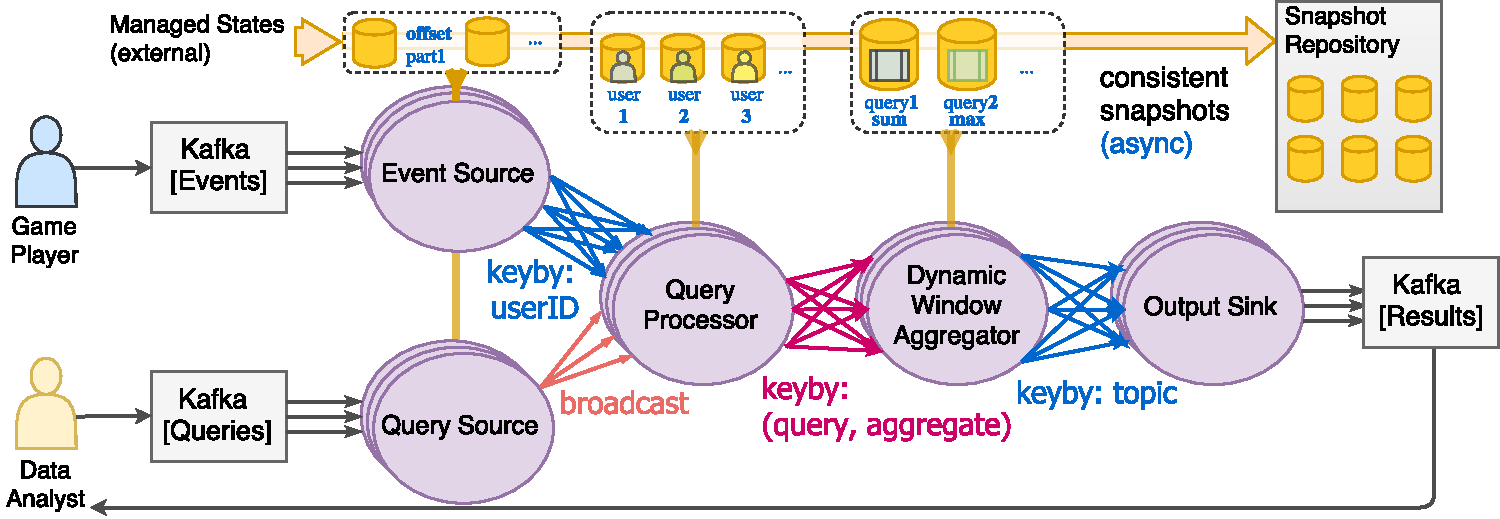
\includegraphics[width=\textwidth]{figures/rbea.pdf}
\caption{Overview of the Flink pipeline implementing an adhoc standing query execution service at King} 
\label{fig:rbea}
\vspace{-4mm}
\end{figure*}



\section{Large-Scale Deployments}
\label{sec:evaluation}

Flink is one of the most widespread open source systems for data stream processing, serving the data processing needs of companies ranging from small startups to large enterprises. It is offered commercially by several vendors, including data Artisans, Lightbend, Amazon AWS, and Google Cloud Platform. A number of companies have published case studies on how they use Flink for stateful stream processing at large scale in the form of blog posts or presentations at industrial conferences and trade shows. For example, {Alibaba}, the world's largest e-commerce retailer company, deploys Flink on over 1000 nodes to support a critical search service \cite{CUSTOM:web/alibaba} and keep search results and recommendation as relevant to their active retail catalogue as possible. {Uber}, the world's largest privately held company at the time of writing is building a stream processing platform based on SQL and Flink, called {AthenaX} \cite{CUSTOM:web/uber} to allow access to timely data to the data scientists in the company. {Netflix} is building a self-serve, scalable, fault-tolerant, multi-tenant “Stream Processing as a Service” platform leveraging Apache Flink with the goal to make the stream of more than 3 petabytes of event data per day available to their internal users \cite{CUSTOM:web/netflix}. Other use cases come from the banking sector \cite{CUSTOM:web/ing}, telecommunications \cite{CUSTOM:web/bouygues} and others \footnote{For the interested reader, the annual Flink Forward series of conferences contains much of these industry presentations \cite{CUSTOM:web/flinkforward} and a recent survey of the Flink community conducted by data Artisans \cite{CUSTOM:web/dartisanssurvey} provides further statistics on how Flink is used within enterprises.}. 

In the remainder of this section, we present live production metrics and insights related to Flink's state management mechanism on a use-case by King (King Digital Entertainment Limited), a leading mobile gaming provider with over 350 million monthly active users.

\subsection{A Real-Time Analytics Platform}

The Rule-Based Event Aggregator (RBEA) by King \cite{CUSTOM:web/kingrbea}, is a reliable live service that is implemented on Apache Flink and used daily by data analysts and developers across the company. RBEA showcases how Flink's stateful processing capabilities can be exploited to build a highly dynamic service that allows analysts to declare and run standing queries on large-scale mobile event streams. In essence, the service covers several fundamental needs of data analysts: 1) instant access to timely user data, 2) the ability to deploy declarative standing queries, 3) creation and manipulation of custom aggregation metrics, 4) a transparent, highly available, consistent execution, eliminating the need for technical expertise.

\subsubsection{The RBEA Service Pipeline}
\autoref{fig:rbea} depicts a simplified overview of the end-to-end Flink pipeline that implements the core of the service. There are two types of streams, ingested from Kafka: a) an \texttt{Event} stream originating from  user actions in the games (over 30 billion events per day) such as \texttt{game\_start/game\_end} and b) a \texttt{Query} stream containing standing queries in the form of serialized scripts written by data analysts through RBEA's frontend in a provided DSL (using Groovy or Java). Standing queries in RBEA allow analysts to access user-specific data and event sequences as well as triggering special aggregation logic on sliding data windows. %(respecting the semantics of Flink's implementation of the Dataflow Model \cite{akidau2015dataflow}). 

Standing queries are forwarded and executed inside \texttt{[Query Processor]} instances which hold managed state entries per user accumulated by any stateful processing logic. A ``broadcast'' data dependency is being used to submit each query to all instances of the \texttt{[Query Processor]} so it can be executed in parallel while game events are otherwise partitioned by their associated user ids to the same operator. Aggregation calls in RBEA's standing query DSL trigger output events from \texttt{[Query Processor]} operator which are subsequently consumed by the \texttt{[Dynamic Window Aggregator]}. This operator assigns the aggregator events to the current event-time window and also applies the actual aggregation logic. Aggregated values are sent to the \texttt{[Output sink]} operator which writes them directly to an external database or Kafka. Some details of the pipeline such as simple stateless filter or projection operators have been omitted to aid understanding as they don't affect state management.

%failures during script execution need to be backpropagated to all the parallel instances in order the remove all instances of the broken scripts. Iterations are used to implement the failure propagation logic.

\begin{figure*}[htp]
\centering
\subcaptionbox{Snapshot Duration vs Total Size \\ \centering [$\pi$:70, \texttt{state}:[100:500GB], \texttt{hosts}:18]}{%
  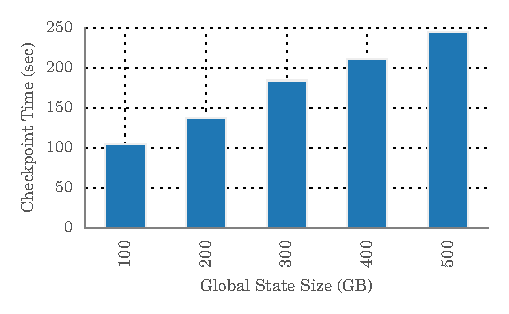
\includegraphics[width=.34\textwidth]{figures/cp1checkpoint.pdf}%
  }\medskip
\subcaptionbox{Alignment Time vs Snapshot Size \\ \centering [$\pi$:70, \texttt{state}:[100:500GB], \texttt{hosts}:18]}{%
  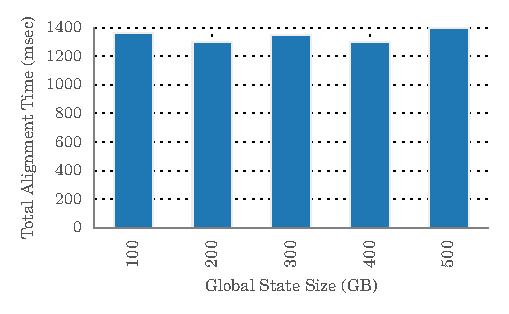
\includegraphics[width=0.34\textwidth]{figures/cp1align.pdf}%
  }\medskip
\subcaptionbox{Alignment Time vs Parallelism \\ \centering [$\pi:[30:70]$, \texttt{state}:200GB, \texttt{hosts}:18]}{%
  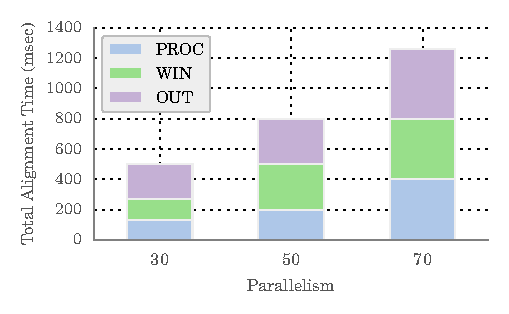
\includegraphics[width=0.34\textwidth]{figures/cp2align.pdf}%
  }
\vspace*{-0.25in}
\caption{RBEA Deployment Measurements on Snapshots }
\label{fig:kingmetrics}
\vspace*{-2mm}
\end{figure*}

\subsubsection{Performance Metrics and Insights} The performance metrics presented here were gathered from live deployments of RBEA over weeks of its runtime in order to present insights and discuss the performance costs related to snapshotting, as well as the factors that can affect those costs in a production setting. The production jobs share resources on a YARN cluster with 18 physical machines with identical specification each having 32 CPU cores, 378 GB RAM with both SSD and HDD. All deployments of RBEA are currently using Flink (v.1.2.0) with local out-of-core RocksDB state backend (on SSD) which enables asynchronous snapshotting to HDFS (backed by HDD). The performance of Flink's state management layer, that we discuss bellow,  has been evaluated to address two main questions: 1) What affects  snapshotting latency?, and 2) How and when is normal execution impacted?
\vspace*{-1mm}

\para{1) What affects snapshotting latency?} \\
We extracted measurements from five different RBEA deployments with fixed parallelism $\pi = 70$ ranging from 100 to 500 GB of global state respectively (each processing data from a specific mobile game). \autoref{fig:kingmetrics}(a) depicts the overall time it takes to undertake a full snapshot asynchronously for different state sizes. Mind that this simply measures the time difference between the invocation of a snapshot (epoch marker injection) and the moment all operators notify back they have completed it through the asynchronous backend calls. As snapshots are asynchronously committed these latencies are not translated into execution impact costs, which makes alignment the sole factor of the snapshotting process that can affect runtime performance (through partial input blocking). \autoref{fig:kingmetrics}(b) shows the overall time RBEA task instances have spent in \emph{alignment} mode, inducing an average delay of 1.3 seconds per full snapshot across all deployments. As expected, there are no indications that alignment times can be affected by the global state size. Given that state is asynchronously snapshotted, normal execution is also not affected by how much state is snapshotted.
\vspace*{-1mm}

\para{2) How and when is normal execution impacted?} \\
Alignment employs partial blocking on input channels of tasks and thus, more connections can introduce higher runtime latency overhead. \autoref{fig:kingmetrics}(c) shows the total times spent aligning per full snapshot in different RBEA deployments of fixed size (200GB) having varying parallelism. Evidently, the number of parallel subtasks $\pi$ affects the alignment time. More concretely, the overall alignment time is proportional to two factors: 1) the number of shuffles chained across the pipeline (i.e., RBEA has 3$\times$ \texttt{keyby} for the \texttt{PROCESSOR}, \texttt{WINDOW} and \texttt{OUTPUT} operators respectively), each of which introduces a form of alignment ``stage'' and 2) the parallelism of the tasks. Nevertheless, occasional latencies of such a low magnitude ($\sim$1sec) are hardly considered to be disruptive or breaking SLAs, especially in highly utilized clusters of such large-scale deployments where network spikes and CPU load can often cause more severe disruptions.



